\documentclass[../opis-rozwiazania.tex]{subfiles}

\begin{document}
\label{state_diagrams}

\subsection{Maszyna wirtualna}
Najważniejszym obiektem biznesowym w systemie jest maszyna wirtualna, do której będą podłączać się użytkownicy.

\begin{figure}[H]
  \centering
  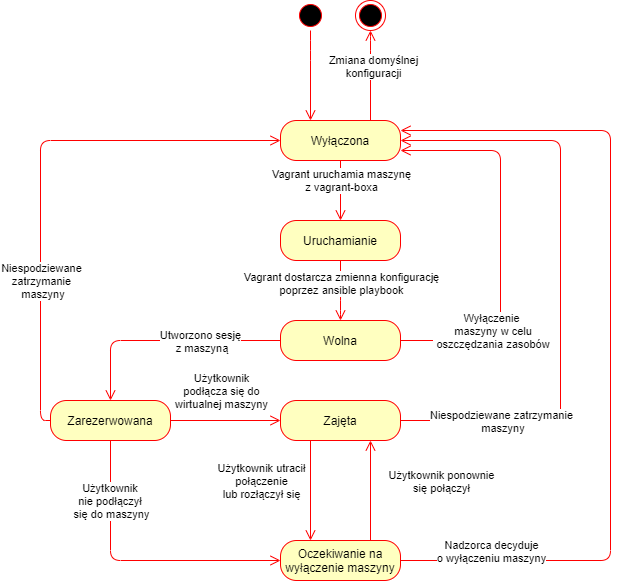
\includegraphics[width=\textwidth]{../diagrams/state_diagrams/virtual_machine.png}
  \caption{Diagram stanów dla maszyny wirtualnej}
  \label{state_vm}
\end{figure}

Maszyna, aby być całkowicie uruchomiona, musi zostać zaopatrzona we wszystkie konfiguracje.
Stan \textit{Wolna} oznacza możliwość przypisania sesji do tej maszyny.
Po przypisaniu maszyny do sesji przechodzi ona w stan oczekiwania na użytkownika. Czas oczekiwania jest konfigurowalny, a po jego upłynięciu maszyna przechodzi w stan oczekiwania na wyłączenie.
W tym stanie oczekuje ona na ponowne połączenie, pozwalając użytkownikowi na bezproblemowy powrót do sesji w przypadku nieoczekiwanego utracenia połączenia. Jeżeli użytkownik nie powróci do sesji, system wyłącza maszynę.
Maszyna jest w stanie \textit{Zajęta}, gdy aktualnie pracuje na niej użytkownik. Monitorowanie zajętości realizowane jest przy użyciu odpowiedniej kolejki wiadomości (rozdział \ref{modules:broker}, kolejka \ref{modules:broker:queue-users}).

\subsection{Serwer wirtualizacji}

Serwer wirtualizacji monitoruje zasoby zużywane przez uruchamiane na nim maszyny wirtualne oraz fakt podłączenia do niego użytkowników.

\begin{figure}[H]
  \centering
  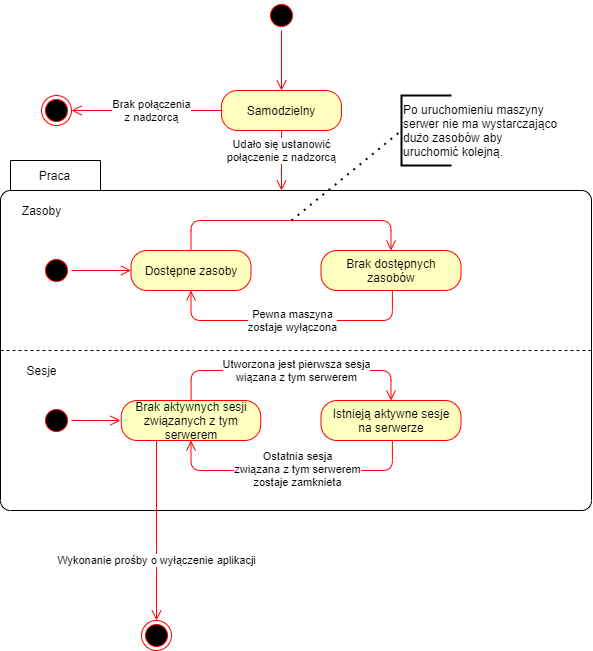
\includegraphics[width=\textwidth]{../diagrams/state_diagrams/virtualisation_server.png}
  \caption{Diagram stanów dla serwera wirtualizacji}
  \label{state_virtsrv}
\end{figure}

Przy starcie serwer wirtualizacji oczekuje na działającego w sieci nadzorcę.
W przypadku jego braku serwer kończy działanie zwracając błąd.
Serwer może mieć wolne zasoby na uruchomienie maszyny lub ich brak.
Jednak ważniejszym stanem z perspektywy działania serwera są podłączeni do niego użytkownicy.
W przypadku gdy podłączony jest do niego przynajmniej jeden użytkownik, serwer nie może poprawnie zakończyć pracy aż użytkownik nie skończy używać maszyny.

\subsection{Użytkownik}

\begin{figure}[H]
  \centering
  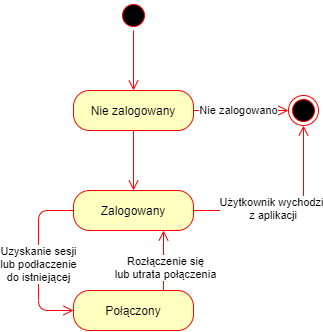
\includegraphics[width=0.6\textwidth]{../diagrams/state_diagrams/client.png}
  \caption{Diagram stanów dla użytkownika}
  \label{state_user}
\end{figure}

Użytkownik z perspektywy systemu po zalogowaniu może być 2 dwóch stanach: pracuje w ramach swojej sesji lub też nie.
W stanie \textit{Połączony} aplikacja kliencka powiadamia serwer wirtualizacji, że ciągle jest obecny.
Przy zmianie stanu do innego informowanie musi ustać, aby serwer mógł wykryć odłączenie się użytkownika.

\end{document}